\subsection*{Level 1}
\addcontentsline{toc}{subsection}{Level 1}


We need to design a discrete time PI-controller which can be used for the following two reference signals.

\begin{enumerate}
 \item Step response to $300$ rad/s :
 \begin{itemize}
  \item[-] As fast as possible;
  \item[-] No overshoot;
  \item[-] Maximum error at steady state $5$ rad/s.
 \end{itemize}
  \item Sine wave reference signal: \\ $vel_{ref} = 300 \sin(0.2t)$ rad/s.
\end{enumerate}

\begin{center} \noindent\rule{6cm}{0.1pt} \end{center}

In this subsection, $T_s = 1 \text{ ms}$.

In order to design the PI-controller, we use the following method:
\begin{itemize}
 \item Add a continuous PI-controller to the model: $C_{PI}(p) = K(1 + \frac{1}{T_i p})$;
 \item Compute the close loop transfer function of the global system;
 \item Design $K,T_i$ such as there is no overshoot and a fast step response;
 \item Discretize the controller;
 \item Redesign $K,T_i$ in order to fulfill the criteria with the discrete controller.
\end{itemize}

% STEP 1
Let the transfer function for the motor be: $$H_{m}(p) = \frac{K_{m}}{1 + \tau_{m} p}$$

The transfer function for the continuous PI-controller is: $$C_{PI}(p) = K\frac{1 + T_i p}{T_i p}$$

% STEP 2
Thus, the close loop transfer function is: \begin{equation} \label{eq1} H_{cl}(p) = \frac{C_{PI}(p) H_{m}(p)}{1 + C_{PI}(p) H_{m}(p)} \end{equation}

Simplifying equation (\ref{eq1}) leads to: 
\begin{multline} \label{contTransfertPI} H_{cl}(p) = \frac{1 + T_i p}{(1+T_i p)(1+\frac{\tau_{m}}{K K_m} p)} \\ - \frac{1 + T_i p}{(T_i + \frac{\tau_m}{K K_m}p) + (T_i + \frac{T_i}{K K_m}p)} \end{multline}
% \begin{equation} \begin{multline} \label{contTransfertPI} H_{cl}(p) = \frac{1 + T_i p}{(1+T_i p)(1+\frac{\tau_{m}}{K K_m} p) - (T_i + \frac{\tau_m}{K K_m}p) + (T_i + \frac{T_i}{K K_m}p)} \end{multline} \end{equation} 

Let \begin{equation} \label{valueTi} T_i = \tau_m \end{equation}

This value leads to a \emph{first order transfer function in closed loop}.

We then have the following transfer function : \begin{equation} H_{cl}(p) = \frac{1}{1 + \frac{\tau_m}{K K_m}p} \end{equation}

% STEP 3
Let $\tau_{s} = \frac{\tau_m}{K K_m}$ be the new time constant of the system.

\begin{description} \item[Remark :] It seems that the bigger $K$ is, the smaller $\tau_{s}$ is. 
  However, we will see that due to saturation limitation that we can not pick whatever value we want. \end{description}

% STEP 4
The continuous transfer function is discretize using Dustin method $\left(p \leftrightarrow \frac{2}{T_s} \frac{1-z^{-1}}{1 + z^{-1}}\right)$ leads to the following transfer function:

\begin{equation} \label{disTransferPI} \frac{K}{2 T_i} \frac{(2 T_i + T_s) + (T_s - 2 T_i) z^{-1} }{ 1 - z^{-1} } \end{equation}

% STEP 5 
$K$ has to be tuned now. Using Simulink, we create a model of the system including the discrete PI-controller. 

We have the following restriction on $U$ : $U(t) \leq 12 \text{ V}$.

Thus, if $K$ gets too big, the output of the PI-controller is saturated. 

We have the following behavior with K too big:

\begin{center}
\begin{tabular}{c}
  $K$ too big \\ 
  $\downarrow$ \\ The PI-controller output is bigger than $12$ V. \\
  $\downarrow$ \\ $U(t)$ is saturated \\
  $\downarrow$ \\ The PI-controller input error can not decrease \\
  $\downarrow$ \\ The integral part of the controller grows to infinity \\
  $\downarrow$ \\ Once the motor has almost reach its final value, the \\saturation disapear and the big integral part leads\\ to an overshoot
\end{tabular}
\end{center}

In order to avoid these behavior, we use the two following solutions:
\begin{itemize}
 \item K is tuned using an iterative method (the biggest value without any overshoot)
 \item The integral part in the PI-controller is saturated ($|U| \leq 7 \text{ V}$) in order to avoid its growing to infinity in case of a saturation of the output.
\end{itemize}

\emph{This analysis leads to the following understanding : 
Even if our system is modelized by a first order system which can theoreticaly has a step response as fast as we want, 
the saturation in the motor input command leads to response velocity limitations.} \ \newline

This behavior is visible on Figure \ref{stepPIspeed}: for each motor input, the rising velocity is the same. 

Figure \ref{stepPIspeed} and \ref{sinPIspeed} display also that our controller fulfill the criteria for the two reference signals -- with a rise time $t_r \leq 50 \text{ ms}$.


Using Matlab, we find the following parameters:
\begin{center}
 \begin{tabular}{|c|c|}
 \hline
 $K$ & $T_i$ (s) \\
 \hline
 $0.13$ & $0.8$ \\
 \hline
 \end{tabular}
\end{center}

\begin{center}
\begin{figure}[ht]
 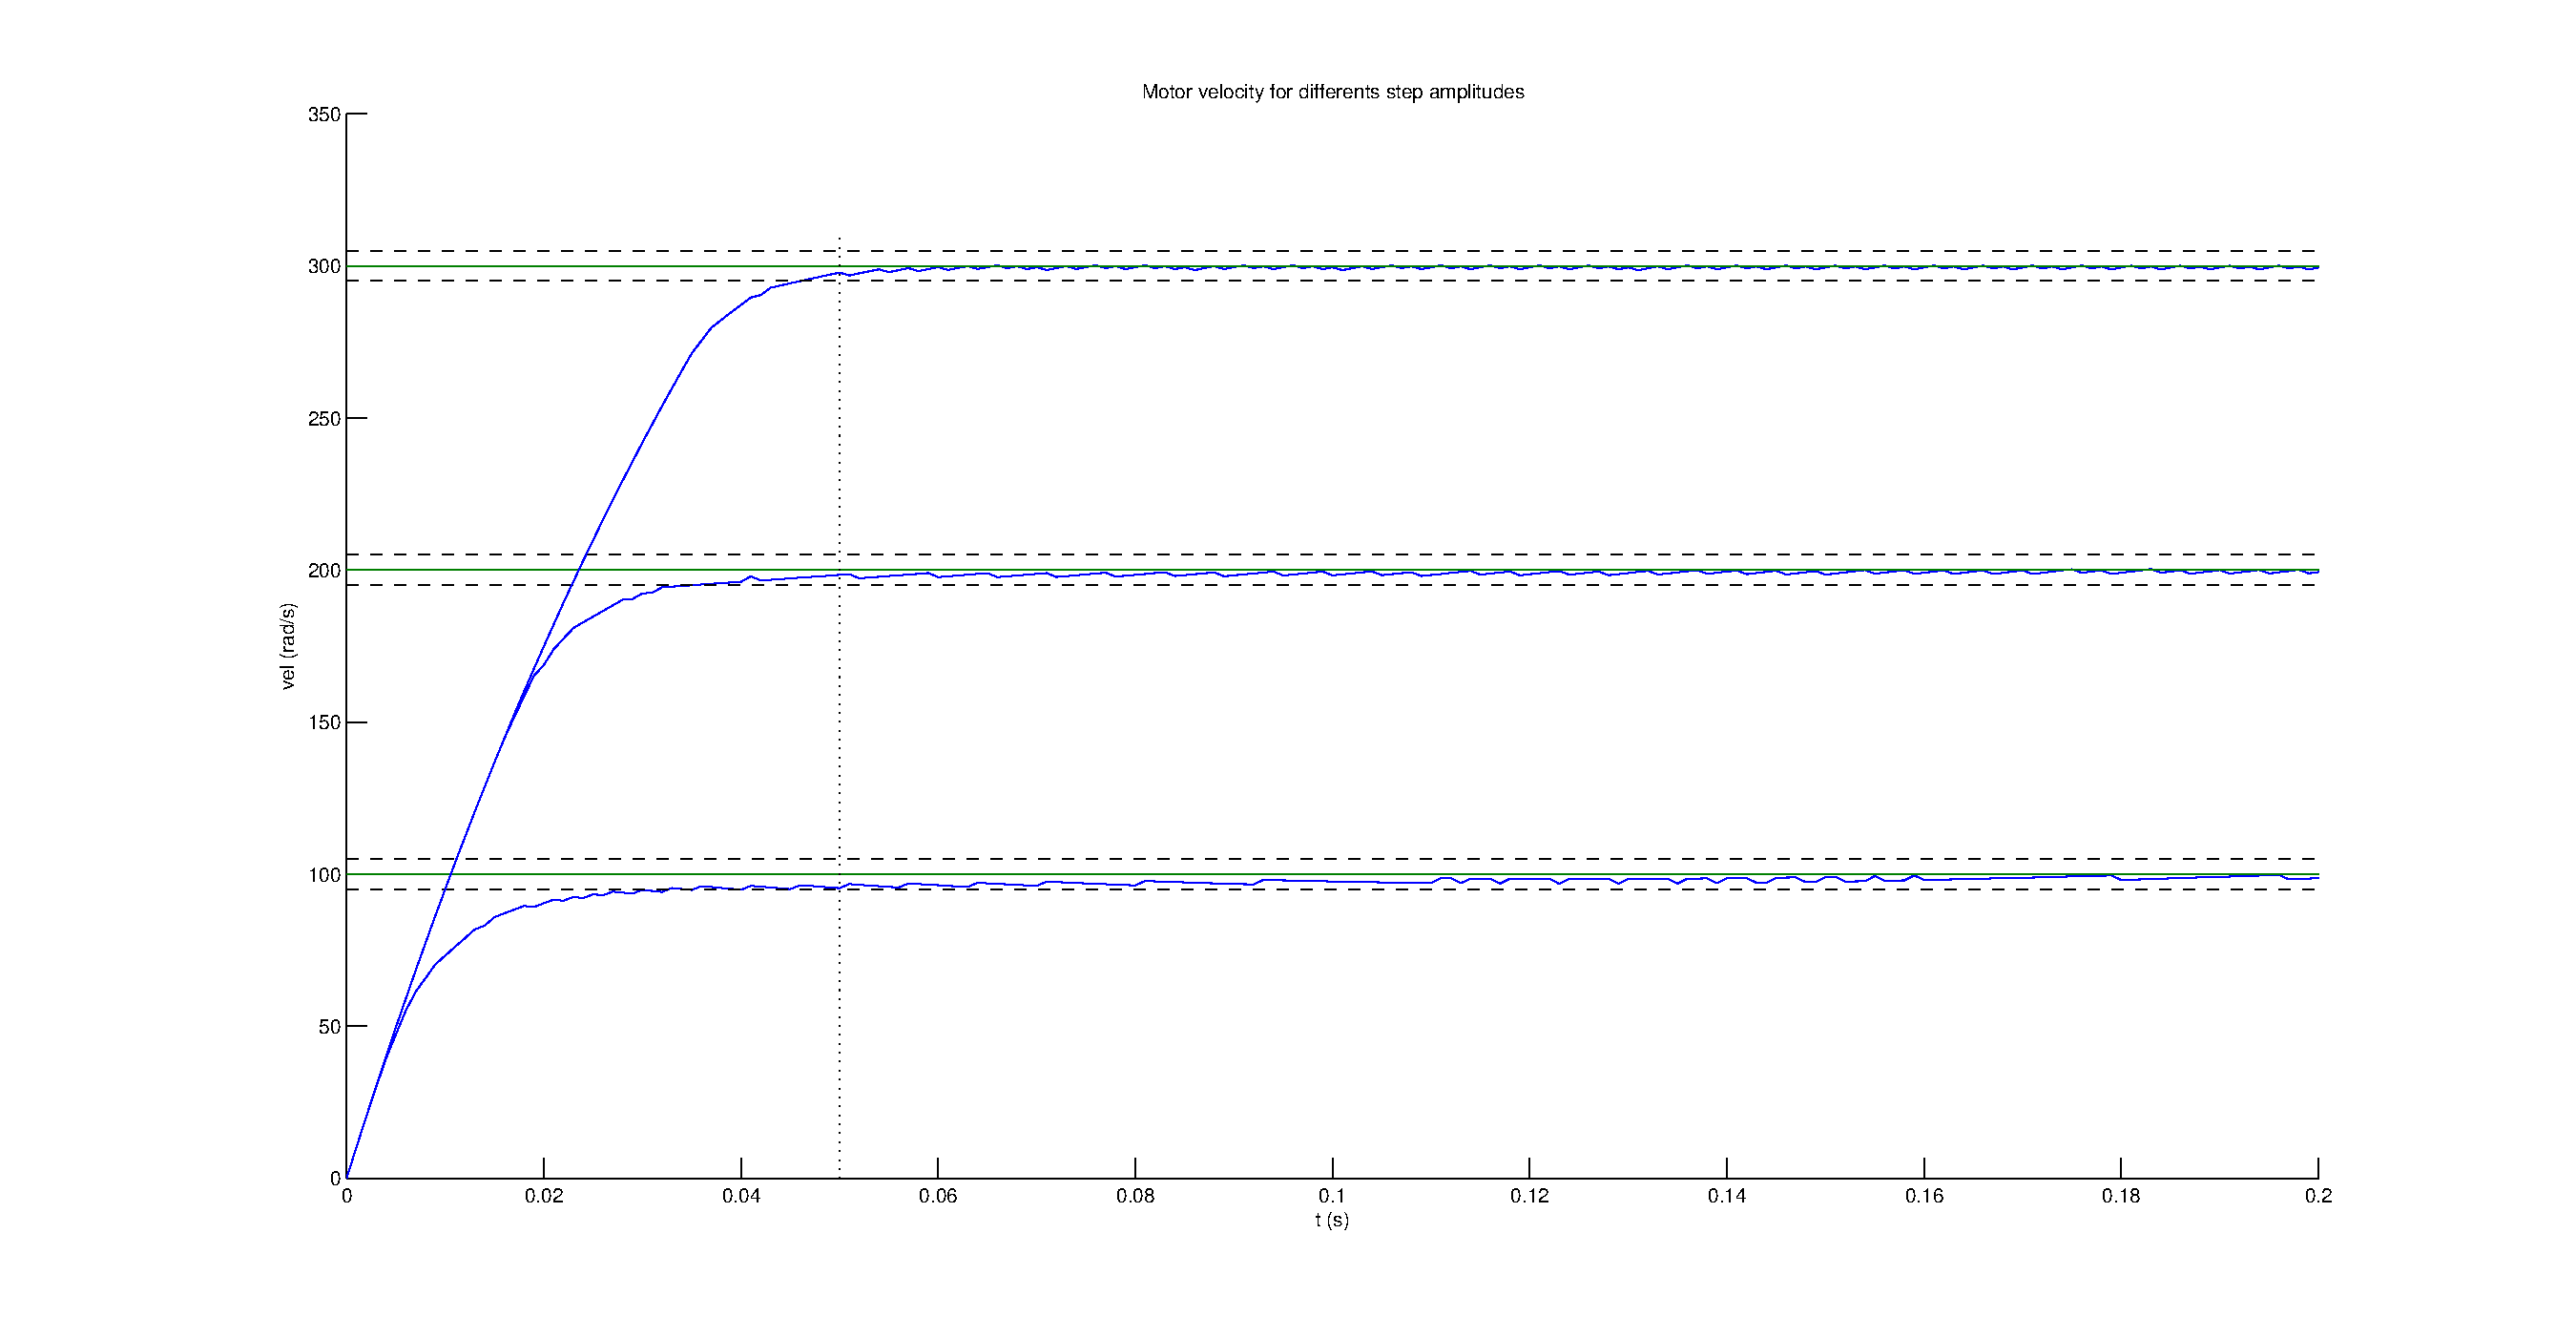
\includegraphics[width=\linewidth]{fig/StepPIspeed.eps}
 \caption{Theoretical motor step response for 3 step input of amplitude $(100,200,300)$ rad/s}
 \label{stepPIspeed}
\end{figure}
\end{center}

\begin{center}
\begin{figure}[ht]
 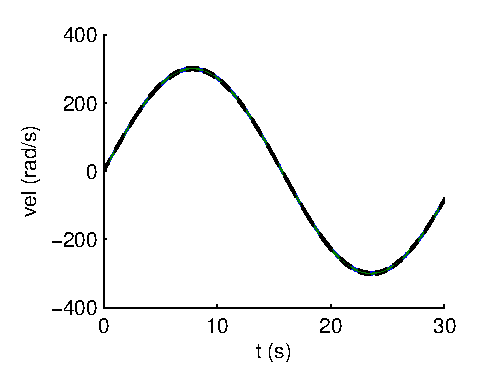
\includegraphics[width=\linewidth]{fig/SinPIspeed.eps}
 \caption{Theoretical motor response for the sine wave reference}
 \label{sinPIspeed}
\end{figure}
\end{center}

